% ============================================================
% FINAL LATEX CODE
% GRN VS. PROPOSED ANATOMY-PRESERVING ULTRASOUND
% SPECKLE DENOISING FRAMEWORK
% ============================================================

\documentclass[conference]{IEEEtran}

% ------------------------------------------------------------
% Packages
% ------------------------------------------------------------
\usepackage{amsmath,amssymb,mathtools}
\usepackage{booktabs}
\usepackage{array}
\usepackage{tabularx}
\usepackage{graphicx}
\usepackage{makecell}

% Vertically centered X columns
\renewcommand{\tabularxcolumn}[1]{m{#1}}

\begin{document}

% ============================================================
% TITLE
% ============================================================

\title{An Anatomy-Preserving Ultrasound Speckle Denoising Framework}

\author{
\IEEEauthorblockN{}
\IEEEauthorblockA{}
}

\maketitle


% ============================================================
% ABSTRACT
% ============================================================

\begin{abstract}
The Generative Reinforcement Network (GRN) is a task-aware framework
designed primarily to improve downstream medical image segmentation
through learned image reconstruction and augmentation. However, its
objective does not explicitly formulate ultrasound speckle denoising
or image-level anatomical boundary preservation. In this work, we
propose an anatomy-preserving ultrasound speckle denoising framework
that explicitly models multiplicative speckle noise and optimizes
pixel-level reconstruction, structural similarity, anatomical edge
preservation, speckle-aware consistency, and downstream segmentation.
Laplacian and frequency-domain losses are considered as optional
extensions and are evaluated through ablation studies. The proposed
framework is designed to evaluate both direct denoising quality and
its effect on downstream anatomical segmentation.
\end{abstract}

\section{Experimental Setup}

The HC18 fetal ultrasound dataset was used to evaluate synthetic speckle denoising performance. Each image was normalized to the range $[0,1]$. Multiplicative Gaussian speckle noise was added using the same degradation model adopted during APD-Net training:

\begin{equation}
I_{\mathrm{noisy}} = I_{\mathrm{clean}} \odot (1+\sigma\epsilon),
\end{equation}

where $\epsilon \sim \mathcal{N}(0,1)$ represents Gaussian noise and $\sigma=0.2$ controls the noise strength. Since paired clean ultrasound images are unavailable, the original HC18 images are considered pseudo-clean references for this synthetic paired evaluation.

\section{Qualitative Comparison}

\begin{figure}[t]
\centering
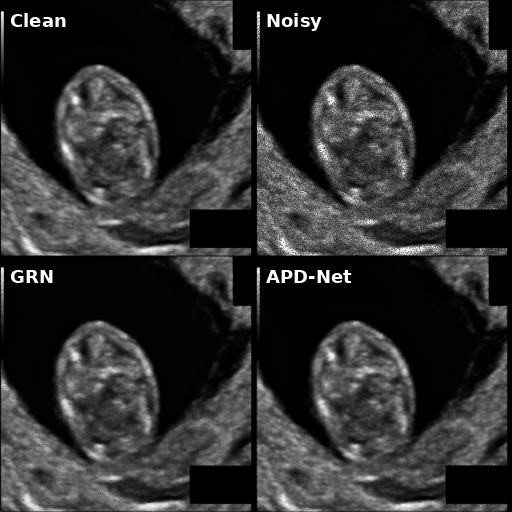
\includegraphics[width=0.95\linewidth]{report_images/hc18_2d/single_image_comparison_5HC_trained_grn.png}
\caption{Qualitative comparison on HC18 sample 5\_HC. The panels show the clean reference image, noisy input, GRN output, and APD-Net output. APD-Net provides improved speckle suppression while maintaining anatomical structures.}
\label{fig:qualitative}
\end{figure}

\section{Quantitative Results}

Table~\ref{tab:results} summarizes the validation performance under synthetic Gaussian speckle noise. The GRN baseline was trained using the same HC18 training split as APD-Net, and both models were evaluated using identical noisy validation samples.

\begin{table}[t]
\centering
\caption{HC18 validation results under synthetic Gaussian speckle noise.}
\label{tab:results}
\resizebox{\linewidth}{!}{
\begin{tabular}{lcccc}
\toprule
Method & PSNR (dB) & SSIM & MAE & Gradient Error \\
\midrule
Noisy & 27.11 & 0.815 & 0.0253 & 0.0363 \\
GRN & 33.64 & 0.927 & 0.0130 & 0.0159 \\
APD-Net & 34.58 & 0.951 & 0.0110 & 0.0141 \\
\bottomrule
\end{tabular}
}
\end{table}

\section{Discussion}

The quantitative and qualitative evaluations indicate that APD-Net improves denoising performance compared with the HC18-trained GRN baseline. APD-Net achieves higher PSNR and SSIM values, indicating improved similarity to the pseudo-clean reference images. Additionally, lower MAE and gradient error values suggest improved preservation of image structures and edge information. These characteristics are important for fetal ultrasound imaging, where maintaining anatomical boundaries is essential for subsequent image analysis applications.

\section{Conclusion}

This study demonstrates the effectiveness of APD-Net for synthetic speckle denoising on HC18 fetal ultrasound images. Compared with the GRN baseline, APD-Net achieves improved reconstruction quality with enhanced structural preservation. The results indicate that APD-Net is a promising approach for ultrasound image restoration and may support downstream analysis tasks.


% ============================================================
% SECTION I
% BACKGROUND AND GRN FORMULATION
% ============================================================

\section{Background: Generative Reinforcement Network (GRN)}

The Generative Reinforcement Network (GRN) is a task-aware framework
that uses a generator $G$, segmentor $S$, and discriminator $D$ to
generate reconstructed images that are beneficial for downstream
segmentation. The reinforcement augmentation (RAug) objective is
formulated as

\begin{equation}
\min_G
\left(
\min_S
L_{\mathrm{seg}}
\left(
S(G(x)),y
\right)
\right),
\qquad
x\sim p_{\mathrm{data}}(x).
\end{equation}

The formulation indicates that the generator is optimized through
the downstream segmentation objective rather than through an explicit
ultrasound speckle-denoising objective.

% ------------------------------------------------------------
% GRN-SEL
% ------------------------------------------------------------

\subsection{GRN-SEL Formulation}

For the Sample-Efficient Learning (GRN-SEL) setting, the generator,
segmentor, and discriminator losses are defined as

\begin{align}
L_G
={}&
\lambda_{\mathrm{adv}}
L_{\mathrm{MSE}}
\left(
D_{\theta'}(\hat I_L),1
\right)
\nonumber\\
&+
\lambda_{\mathrm{seg}}
L_{\mathrm{Dice}}
\left(
\hat M_L,M
\right)
+
\lambda_{L1}
L_1
\left(
\hat I_L,I_L
\right),
\end{align}

\begin{equation}
L_S
=
\frac{
L_{\mathrm{Dice}}(M_L,M)
+
L_{\mathrm{Dice}}(\hat M_L,M)
}{2},
\end{equation}

and

\begin{equation}
L_D
=
\frac{
L_{\mathrm{MSE}}
\left(
D_{\theta'}(I_L),1
\right)
+
L_{\mathrm{MSE}}
\left(
D_{\theta'}(\hat I_L),0
\right)
}{2}.
\end{equation}

Thus, the GRN-SEL generator objective combines adversarial,
segmentation, and pixel-level $L_1$ reconstruction terms.

% ------------------------------------------------------------
% GRN-SSL
% ------------------------------------------------------------

\subsection{GRN-SSL Formulation}

In the Semi-Supervised Learning (GRN-SSL) setting, GRN additionally
uses a customized consistency objective. The interpolation consistency
term can be represented as

\begin{equation}
L_{\mathrm{ICT}}
=
\mathrm{MSE}
\left(
M_{\mathrm{mixed}},
\mathrm{Mix}_{\lambda}
(M_{\mathrm{UL}},M_S)
\right),
\end{equation}

where

\begin{equation}
\mathrm{Mix}_{\lambda}(T_a,T_b)
=
\lambda T_a+(1-\lambda)T_b.
\end{equation}

Therefore, GRN-SEL and GRN-SSL should be distinguished when describing
the complete GRN framework.


% ============================================================
% SECTION II
% PROPOSED FRAMEWORK
% ============================================================

\section{Proposed Anatomy-Preserving Denoising Framework}

The proposed framework changes the optimization target from
segmentation-oriented image generation to explicit ultrasound
speckle denoising with anatomical preservation and downstream
segmentation consistency.

The denoising generator is defined as

\begin{equation}
\hat I
=
G_{\theta}
\left(
I_{\mathrm{noisy}}
\right),
\end{equation}

where $\hat I$ denotes the denoised ultrasound image.

Unlike GRN, the proposed framework explicitly considers the
multiplicative nature of ultrasound speckle:

\begin{equation}
I_{\mathrm{noisy}}
=
I_{\mathrm{clean}}
\odot N_s,
\label{eq:speckle_model}
\end{equation}

where $N_s$ represents the multiplicative speckle component and
$\odot$ denotes the Hadamard product.


% ============================================================
% SECTION III
% TABLE 1
% ============================================================

\begin{table*}[t]
\centering
\caption{Limitations of GRN and corresponding solutions in the proposed ultrasound speckle denoising framework.}
\label{tab:grn_limitations}

\renewcommand{\arraystretch}{1.45}
\setlength{\tabcolsep}{5pt}

\begin{tabularx}{\textwidth}{
    >{\raggedright\arraybackslash}m{0.27\textwidth}
    >{\raggedright\arraybackslash}m{0.28\textwidth}
    >{\raggedright\arraybackslash}X
}
\toprule

\textbf{What GRN lacks}
&
\textbf{What our new method solves}
&
\textbf{How it solves the problem}
\\

\midrule

No explicit ultrasound speckle-noise model
&
Explicit ultrasound speckle modeling
&
Models ultrasound speckle as approximately multiplicative noise,
$I_{\mathrm{noisy}}
=
I_{\mathrm{clean}}\odot N_s$,
and introduces a logarithmic-domain speckle-aware loss.
\\

Denoising is not the primary objective
&
Direct ultrasound denoising becomes the primary objective
&
The generator is explicitly trained to reconstruct a denoised image
using pixel, structural, anatomical, and speckle-aware objectives.
\\

No explicit SSIM-based structural constraint
&
Explicit structural preservation
&
Introduces
$L_{\mathrm{SSIM}}
=
1-\mathrm{SSIM}(\hat I,I_{\mathrm{ref}})$
to preserve image-level structural similarity.
\\

No explicit image-level anatomical edge-preservation loss
&
Explicit anatomical boundary preservation
&
Uses a gradient-based loss to penalize differences between the
anatomical edge structures of the output and reference image.
\\

No explicit second-order structural constraint
&
Optional fine-structure preservation
&
Introduces a Laplacian loss as an experimentally evaluated extension,
rather than assuming that stronger high-frequency preservation always
improves denoising.
\\

No explicit frequency-domain objective
&
Optional frequency-aware preservation
&
Introduces a frequency-domain loss as an ablation component and
evaluates whether frequency preservation improves anatomical
information without retaining unwanted speckle.
\\

Segmentation-oriented optimization does not explicitly optimize
ultrasound denoising quality
&
Segmentation becomes a downstream anatomical constraint
&
Retains segmentation feedback while making direct denoising and
anatomical preservation explicit objectives.
\\

No direct denoising evaluation as the primary objective
&
Direct quantitative denoising evaluation
&
Evaluates PSNR, SSIM, MAE, and MSE for synthetic paired experiments,
together with SNR, CNR, ENL, and edge-preservation measures where
appropriate.
\\

Limited external validation on another 3-D ultrasound cLBP dataset
&
Cross-dataset evaluation
&
Tests whether the learned denoising representation generalizes across
different ultrasound datasets and anatomical regions where suitable
datasets are available.
\\

Inference-time computational overhead from SGE
&
Explicit computational-efficiency evaluation
&
Reports parameter count, FLOPs, inference time, and GPU memory in
addition to denoising and segmentation performance.
\\

\bottomrule
\end{tabularx}
\end{table*}


% ============================================================
% SECTION IV
% TABLE 2
% ============================================================

\begin{table*}[t]
\centering
\caption{Mathematical comparison between GRN and the proposed anatomy-preserving ultrasound speckle denoising framework.}
\label{tab:grn_vs_proposed}

\renewcommand{\arraystretch}{1.55}
\setlength{\tabcolsep}{4pt}

\begin{tabularx}{\textwidth}{
    >{\raggedright\arraybackslash}m{0.15\textwidth}
    >{\raggedright\arraybackslash}m{0.25\textwidth}
    >{\raggedright\arraybackslash}m{0.21\textwidth}
    >{\raggedright\arraybackslash}X
}
\toprule

\textbf{Component}
&
\textbf{GRN formulation}
&
\textbf{Proposed change}
&
\textbf{Proposed formulation}
\\

\midrule

Generator output
&
\[
\hat I=G(I)
\]
&
Explicitly formulate the generator as a denoiser
&
\[
\hat I
=
G_{\theta}
(I_{\mathrm{noisy}})
\]
\\

Primary GRN-SEL generator objective
&
\[
\begin{aligned}
L_G={}&
\lambda_{\mathrm{adv}}L_{\mathrm{adv}}
+
\lambda_{\mathrm{seg}}L_{\mathrm{seg}}
\\
&+
\lambda_{L1}L_1
\end{aligned}
\]
&
Replace the segmentation-oriented image-generation objective with an
explicit denoising objective
&
\[
\begin{aligned}
L_{\mathrm{total}}
={}&
\lambda_{\mathrm{pix}}L_{\mathrm{pix}}
+
\lambda_{\mathrm{SSIM}}L_{\mathrm{SSIM}}
\\
&+
\lambda_{\mathrm{edge}}L_{\mathrm{edge}}
+
\lambda_{\mathrm{speckle}}L_{\mathrm{speckle}}
\\
&+
\lambda_{\mathrm{seg}}L_{\mathrm{seg}}
\end{aligned}
\]
\\

Adversarial loss
&
\[
L_{\mathrm{adv}}
=
L_{\mathrm{MSE}}
\left(
D(\hat I),1
\right)
\]
&
Not required as the primary denoising objective
&
Adversarial loss is omitted from the core formulation and can be
evaluated as an optional extension.
\\

Pixel reconstruction
&
\[
L_1
=
\|\hat I-I\|_1
\]
&
Retain pixel-level reconstruction as one component
&
\[
L_{\mathrm{pix}}
=
\frac{1}{N}
\left\|
\hat I-I_{\mathrm{ref}}
\right\|_1
\]
\\

Segmentation loss
&
\[
L_{\mathrm{seg}}
=
L_{\mathrm{Dice}}
\left(
S(\hat I),M
\right)
\]
&
Retain segmentation feedback as a downstream anatomical constraint
&
\[
L_{\mathrm{seg}}
=
1-
\frac{
2\sum_i\hat M_iM_i+\epsilon
}{
\sum_i\hat M_i+\sum_iM_i+\epsilon
}
\]
\\

Speckle model
&
No explicit speckle model in the GRN objective
&
Introduce an ultrasound-specific multiplicative speckle model
&
\[
I_{\mathrm{noisy}}
=
I_{\mathrm{clean}}
\odot N_s
\]
\\

Speckle-aware loss
&
Not explicitly defined
&
Introduce a loss specifically related to multiplicative speckle
&
\[
L_{\mathrm{speckle}}
=
\frac{1}{N}
\left\|
\log(\hat I+\epsilon)
-
\log(I_{\mathrm{ref}}+\epsilon)
\right\|_1
\]
\\

SSIM loss
&
Not explicitly included in the generator objective
&
Explicitly preserve structural similarity
&
\[
L_{\mathrm{SSIM}}
=
1-
\mathrm{SSIM}
(\hat I,I_{\mathrm{ref}})
\]
\\

Anatomical edge preservation
&
No explicit image-level gradient loss
&
Explicitly preserve anatomical boundaries
&
\[
L_{\mathrm{edge}}
=
\frac{1}{N}
\left\|
\nabla\hat I
-
\nabla I_{\mathrm{ref}}
\right\|_1
\]
\\

Laplacian preservation
&
No explicit second-order structural loss
&
Evaluate fine-structure preservation as an optional extension
&
\[
L_{\mathrm{lap}}
=
\frac{1}{N}
\left\|
\nabla^2\hat I
-
\nabla^2I_{\mathrm{ref}}
\right\|_1
\]
\\

Frequency preservation
&
No explicit frequency-domain objective
&
Evaluate frequency preservation as an optional extension
&
\[
L_{\mathrm{freq}}
=
\left\|
W(f)
\left[
|\mathcal{F}(\hat I)|
-
|\mathcal{F}(I_{\mathrm{ref}})|
\right]
\right\|_1
\]
\\

Primary optimization target
&
Segmentation-oriented image generation
&
Explicit denoising + anatomical preservation + downstream segmentation
&
\[
\hat I
=
\arg\min_G
\left(
L_{\mathrm{denoise}}
+
L_{\mathrm{structure}}
+
L_{\mathrm{seg}}
\right)
\]
\\

Final core objective
&
\[
\boxed{
L_{\mathrm{GRN\text{-}SEL}}
=
\lambda_{\mathrm{adv}}L_{\mathrm{adv}}
+
\lambda_{\mathrm{seg}}L_{\mathrm{seg}}
+
\lambda_{L1}L_1
}
\]
&
Multi-objective ultrasound denoising
&
\[
\boxed{
\begin{aligned}
L_{\mathrm{total}}
={}&
\lambda_{\mathrm{pix}}L_{\mathrm{pix}}
+
\lambda_{\mathrm{SSIM}}L_{\mathrm{SSIM}}
\\
&+
\lambda_{\mathrm{edge}}L_{\mathrm{edge}}
+
\lambda_{\mathrm{speckle}}L_{\mathrm{speckle}}
\\
&+
\lambda_{\mathrm{seg}}L_{\mathrm{seg}}
\end{aligned}
}
\]
\\

\bottomrule
\end{tabularx}
\end{table*}


% ============================================================
% SECTION V
% PROPOSED CORE OBJECTIVE
% ============================================================

\section{Proposed Core Objective Function}

The proposed core objective explicitly combines pixel-level
reconstruction, structural similarity, anatomical edge preservation,
speckle-aware consistency, and downstream segmentation:

\begin{equation}
\boxed{
\begin{aligned}
L_{\mathrm{total}}
={}&
\lambda_{\mathrm{pix}}L_{\mathrm{pix}}
+
\lambda_{\mathrm{SSIM}}L_{\mathrm{SSIM}}
\\
&+
\lambda_{\mathrm{edge}}L_{\mathrm{edge}}
+
\lambda_{\mathrm{speckle}}L_{\mathrm{speckle}}
\\
&+
\lambda_{\mathrm{seg}}L_{\mathrm{seg}}.
\end{aligned}
}
\label{eq:proposed_total_loss}
\end{equation}


% ============================================================
% PIXEL LOSS
% ============================================================

\subsection{Pixel Reconstruction Loss}

The pixel-level reconstruction loss is defined as

\begin{equation}
L_{\mathrm{pix}}
=
\frac{1}{N}
\left\|
\hat I-I_{\mathrm{ref}}
\right\|_1.
\label{eq:pixel_loss}
\end{equation}


% ============================================================
% SSIM LOSS
% ============================================================

\subsection{Structural Similarity Loss}

Structural preservation is encouraged using the SSIM loss:

\begin{equation}
L_{\mathrm{SSIM}}
=
1-
\mathrm{SSIM}
\left(
\hat I,I_{\mathrm{ref}}
\right).
\label{eq:ssim_loss}
\end{equation}


% ============================================================
% EDGE LOSS
% ============================================================

\subsection{Anatomical Edge-Preservation Loss}

To explicitly preserve anatomical boundaries, a first-order gradient
loss is introduced:

\begin{equation}
L_{\mathrm{edge}}
=
\frac{1}{N}
\left\|
\nabla\hat I
-
\nabla I_{\mathrm{ref}}
\right\|_1.
\label{eq:edge_loss}
\end{equation}


% ============================================================
% SPECKLE-AWARE LOSS
% ============================================================

\subsection{Speckle-Aware Loss}

Under the multiplicative speckle model

\begin{equation}
I_{\mathrm{noisy}}
=
I_{\mathrm{clean}}
\odot N_s,
\end{equation}

taking the logarithm transforms the multiplicative relationship
into an additive form:

\begin{equation}
\log(I_{\mathrm{noisy}}+\epsilon)
\approx
\log(I_{\mathrm{clean}}+\epsilon)
+
\log(N_s+\epsilon).
\end{equation}

The proposed logarithmic-domain speckle-aware loss is

\begin{equation}
L_{\mathrm{speckle}}
=
\frac{1}{N}
\left\|
\log(\hat I+\epsilon)
-
\log(I_{\mathrm{ref}}+\epsilon)
\right\|_1.
\label{eq:speckle_loss}
\end{equation}


% ============================================================
% SEGMENTATION LOSS
% ============================================================

\subsection{Downstream Segmentation Loss}

Segmentation is retained as a downstream anatomical constraint rather
than as the sole definition of image quality. The soft Dice loss is

\begin{equation}
L_{\mathrm{seg}}
=
1-
\frac{
2\sum_i\hat M_iM_i+\epsilon
}{
\sum_i\hat M_i+\sum_iM_i+\epsilon
}.
\label{eq:dice_loss}
\end{equation}


% ============================================================
% OPTIONAL EXTENSIONS
% ============================================================

\section{Optional Structural Extensions}

The following terms are not assumed to improve denoising a priori.
They are treated as experimentally evaluated extensions and should
be validated through ablation studies.

% ------------------------------------------------------------
% LAPLACIAN LOSS
% ------------------------------------------------------------

\subsection{Laplacian Fine-Structure Loss}

An optional second-order loss is defined as

\begin{equation}
L_{\mathrm{lap}}
=
\frac{1}{N}
\left\|
\nabla^2\hat I
-
\nabla^2I_{\mathrm{ref}}
\right\|_1.
\label{eq:lap_loss}
\end{equation}

Because the Laplacian emphasizes high-frequency information, its
effect on both anatomical detail preservation and speckle suppression
must be experimentally evaluated.

% ------------------------------------------------------------
% FREQUENCY LOSS
% ------------------------------------------------------------

\subsection{Frequency-Domain Loss}

An optional frequency-domain loss is defined as

\begin{equation}
L_{\mathrm{freq}}
=
\left\|
W(f)
\left[
|\mathcal{F}(\hat I)|
-
|\mathcal{F}(I_{\mathrm{ref}})|
\right]
\right\|_1,
\label{eq:frequency_loss}
\end{equation}

where $W(f)$ is a frequency-dependent weighting function.

The weighting function can be used to avoid indiscriminately
preserving high-frequency components that may contain unwanted
speckle.


% ============================================================
% EXTENDED OBJECTIVE
% ============================================================

\subsection{Extended Objective}

When validated through ablation experiments, the optional Laplacian
and frequency-domain terms can be incorporated into the core objective:

\begin{equation}
\boxed{
\begin{aligned}
L_{\mathrm{extended}}
={}&
L_{\mathrm{total}}
+
\lambda_{\mathrm{lap}}L_{\mathrm{lap}}
+
\lambda_{\mathrm{freq}}L_{\mathrm{freq}}.
\end{aligned}
}
\label{eq:extended_loss}
\end{equation}


% ============================================================
% HC18 REFERENCE IMAGE DEFINITION
% ============================================================

\section{Reference Image Definition for HC18}

The HC18 dataset does not provide paired noise-free and noisy
ultrasound images. Therefore, when synthetic multiplicative speckle
is applied to an original HC18 image, the original image is treated
as a \textit{pseudo-clean reference} rather than a true noise-free
ground-truth image.

Specifically,

\begin{equation}
I_{\mathrm{HC18}}
\rightarrow
I_{\mathrm{noisy}}
=
I_{\mathrm{HC18}}
\odot N_s,
\end{equation}

where the original image $I_{\mathrm{HC18}}$ is used as the
pseudo-clean reference for the synthetic paired denoising experiment.

Accordingly, the notation

\begin{equation}
I_{\mathrm{ref}}
=
I_{\mathrm{HC18}}
\end{equation}

denotes the pseudo-clean reference in the HC18 synthetic-speckle
setting.


% ============================================================
% NOTATION
% ============================================================

\section{Notation and Parameter Definitions}

\begin{itemize}

    \item $\hat I$: Denoised ultrasound image produced by the
    generator, $\hat I=G_{\theta}(I_{\mathrm{noisy}})$.

    \item $I_{\mathrm{noisy}}$: Ultrasound image corrupted by
    multiplicative speckle noise.

    \item $I_{\mathrm{clean}}$: Underlying noise-free ultrasound
    image in the mathematical speckle model.

    \item $I_{\mathrm{ref}}$: Reference image used for the denoising
    objective. In HC18 synthetic experiments, it denotes the
    pseudo-clean original image.

    \item $N_s$: Multiplicative ultrasound speckle component.

    \item $\hat M_i$: Predicted soft segmentation probability at
    spatial location $i$.

    \item $M_i$: Ground-truth segmentation label at spatial
    location $i$.

    \item $N$: Number of pixels or voxels in the image domain.

    \item $\lambda_{\mathrm{pix}}$: Weight of the pixel reconstruction
    loss.

    \item $\lambda_{\mathrm{SSIM}}$: Weight of the structural
    similarity loss.

    \item $\lambda_{\mathrm{edge}}$: Weight of the anatomical
    edge-preservation loss.

    \item $\lambda_{\mathrm{speckle}}$: Weight of the speckle-aware
    loss.

    \item $\lambda_{\mathrm{seg}}$: Weight of the downstream
    segmentation loss.

    \item $\lambda_{\mathrm{lap}}$: Weight of the optional
    Laplacian loss.

    \item $\lambda_{\mathrm{freq}}$: Weight of the optional
    frequency-domain loss.

    \item $\nabla$: First-order spatial gradient operator.

    \item $\nabla^2$: Second-order Laplacian operator.

    \item $\mathcal{F}(\cdot)$: Fourier transform operator.

    \item $|\cdot|$: Magnitude operator.

    \item $\odot$: Hadamard element-wise product.

    \item $\|\cdot\|_1$: Element-wise $L_1$ norm.

    \item $\epsilon$: Small positive constant used for numerical
    stability.

    \item $W(f)$: Frequency-dependent weighting function.

\end{itemize}


% ============================================================
% CONCEPTUAL SUMMARY
% ============================================================

\section{Conceptual Difference}

The fundamental difference between GRN and the proposed framework
can be summarized as

\begin{equation}
\boxed{
\mathrm{GRN}
\quad\rightarrow\quad
\text{Segmentation-oriented image generation}
}
\end{equation}

whereas the proposed framework is formulated as

\begin{equation}
\boxed{
\mathrm{Proposed\ Method}
\quad\rightarrow\quad
\text{Speckle denoising}
+
\text{Anatomical preservation}
+
\text{Downstream segmentation}
}
\end{equation}

The central research hypothesis is therefore that explicit modeling
of ultrasound speckle and anatomical structure can produce
quantitatively improved denoising while preserving or improving
downstream segmentation performance.


\end{document}